\begin{figure}[htbp]
    \centering
    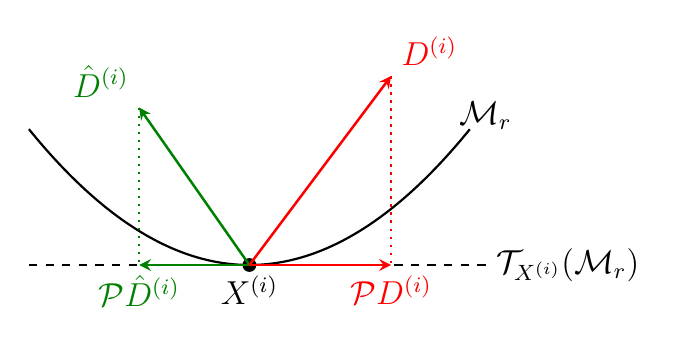
\begin{tikzpicture}[
        >=stealth,
        line width=0.9pt,
        every node/.style={font=\large}
    ]
    % Manifold M_r as a smooth curve
    \draw[thick] plot[smooth, domain=-2.8:2.8, samples=60]
        ({\x}, {0.22*\x*\x - 1});
    \node at (3, 0.9) {$\mathcal{M}_r$};

    % Tangent line at X^(i)
    \draw[dashed] (-2.8, -1) -- (3, -1);
    \node[right] at (3, -1) {$\mathcal{T}_{X^{(i)}}(\mathcal{M}_r)$};

    % Point X^(i)
    \coordinate (X) at (0, -1);
    \fill (X) circle (2.5pt);
    \node[below] at (X) {$X^{(i)}$};

    % \hat D^(i) = -grad Phi(X^(i)): true steepest descent direction at X^(i)
    \coordinate (Dhat) at (-1.4, 1);
    \draw[->, Green] (X) -- (Dhat);
    \node[above left, Green] at (Dhat) {$\hat D^{(i)}$};

    % Dotted projection from \hat D tip down onto the tangent line
    \draw[dotted, Green] (Dhat) -- (-1.4, -1);

    % P \hat D^(i): projection of \hat D onto T_{X^(i)} M_r (Riemannian descent direction)
    \coordinate (PDhat) at (-1.4, -1);
    \draw[->, Green] (X) -- (PDhat);
    \node[below, Green] at (PDhat) {$\mathcal{P}\hat D^{(i)}$};

    % D^(i): CG search direction, generated by the recurrence
    \coordinate (D) at (1.8, 1.4);
    \draw[->, Red] (X) -- (D);
    \node[above right, Red] at (D) {$D^{(i)}$};

    % Dotted projection from D tip down onto the tangent line
    \draw[dotted, Red] (D) -- (1.8, -1);

    % P D^(i): projection of D onto T_{X^(i)} M_r
    \coordinate (PD) at (1.8, -1);
    \draw[->, Red] (X) -- (PD);
    \node[below, Red] at (PD) {$\mathcal{P}D^{(i)}$};

    \end{tikzpicture}
    \caption{The CG search direction $D^{(i)}$ may disagree with the steepest-descent direction $\hat D^{(i)} = -\nabla\Phi(X^{(i)})$, so that their projections $\mathcal{P}D^{(i)}$ and $\mathcal{P}\hat D^{(i)}$ onto the tangent space $\mathcal{T}_{X^{(i)}}(\mathcal{M}_r)$ point in very different directions.}
    \label{fig:cg_direction_disagreement}
\end{figure}